\section{Sequences and series}

\subsection{What is a sequence?}

A \textit{sequence} is essentially an ordered list of numbers. Examples include the harmonic sequence and the Fibonacci sequence, both of which are shown below.
%
\begin{align}
    & 1, \frac{1}{2}, \frac{1}{3}, \frac{1}{4}, \frac{1}{5}, \cdots\tag{Harmonic sequence}\\
    &\notag\\
    & 0, 1, 1, 2, 3, 5, 8, 13, \cdots \tag{Fibonacci sequence}
\end{align}
%
We denote the sequence \(u_0, u_1, u_2, u_3, \cdots\) as \((u_n)\), with \(n \in \mathbb{N}\). Note that zero-based indexing is used here.

For instance, we can define the harmonic sequence using
%
\[u_n = \frac{1}{n+1}\]
%
while the Fibonacci sequence can be described by the recurrence relation
%
\[u_{n+2} = u_{n+1} + u_n\text{.}\]



\subsection{Arithmetic, geometric, monotone, bounded and recursive sequences}

An \textit{arithmetic sequence} is one where each term is obtained by adding a constant increment \(d\) to the previous term. The general term of an arithmetic sequence \((u_n)\) is given by
%
\[u_n = a + nd\]
%
where \(a = u_0\) is the first term of the sequence.

A \textit{geometric sequence} is one where each term is obtained by multiplying the previous term by a constant ratio \(r\). The general term of a geometric sequence \((u_n)\) is given by
%
\[u_n = a r^n\]
%
where \(a = u_0\) is the first term of the sequence.


\begin{figure}[H]
    \centering

    \begin{tikzpicture}[scale=0.75]
        \draw[thin,gray!40] (-1,-1) grid (8, 5);
        \draw[thick, ->, >=latex] (-1,0)--(8,0) node[right]{\(x\)};
        \draw[thick, ->, >=latex] (0,-1)--(0,5) node[above]{\(y\)};
        \draw (0, 0) node[below left] {0};

        \draw [MidnightBlue, very thick, domain=-1:8, samples=100] plot (\x,{0.5*\x + 1});

        \foreach \x in {0,1,...,8} {
            \filldraw[MidnightBlue] (\x, 0.5*\x+1) circle [radius=3pt];
        }

        \draw (4, 2) node[above right, MidnightBlue] {\(u_n = \dfrac{1}{2} n + 1\)};
    \end{tikzpicture}
    
    \caption{The graph of an arithmetic sequence.}
    \label{fig:Ch05-arithmetic-seq-graph}
\end{figure}



\begin{figure}[H]
    \centering

    \begin{tikzpicture}[scale=0.75]
        \draw[thin,gray!40] (-1,-1) grid (8, 9);
        \draw[thick, ->, >=latex] (-1,0)--(8,0) node[right]{\(x\)};
        \draw[thick, ->, >=latex] (0,-1)--(0,9) node[above]{\(y\)};
        \draw (0, 0) node[below left] {0};

        \draw [MidnightBlue, very thick, domain=-1:8, samples=100] plot (\x,{2 * 1.2^\x});

        \foreach \x in {0,1,...,8} {
            \filldraw[MidnightBlue] (\x, 2 * 1.2^\x) circle [radius=3pt];
        }

        \draw (4.3, 3) node[above right, MidnightBlue] {\(u_n = 2 \cdot \left(\dfrac{6}{5}\right)^n\)};
    \end{tikzpicture}
    
    \caption{The graph of an geometric sequence.}
    \label{fig:Ch05-geometric-seq-graph}
\end{figure}




A sequence \((u_n)\) is said to be...
%
\begin{itemize}
    \item ...\textit{increasing} if for all \(n \in \mathbb{N}\), we have \(u_{n+1} \geq u_n\).
    \item ...\textit{decreasing} if for all \(n \in \mathbb{N}\), we have \(u_{n+1} \leq u_n\).
    \item ...\textit{monotone} if it is either increasing or decreasing.
    \item ...\textit{bounded} if there exists some real number \(M\) such that for all \(n \in \mathbb{N}\), we have \(\abs{u_n} \leq M\).
\end{itemize}

Notice that in non-strict inequalities (as opposed to strict inequalities) are used in the first two definitions. This means that a constant sequence is both increasing and decreasing.

In the last definition, both strict or non-strict inequalities can be used --- they are equivalent in this context.



\begin{figure}[H]
    \centering

    \begin{tikzpicture}[scale=0.9]
        \draw[thin,gray!40] (-1,-2) grid (8, 3);
        \draw[thick, ->, >=latex] (-1,0)--(8,0) node[right]{\(x\)};
        \draw[thick, ->, >=latex] (0,-2)--(0,3) node[above]{\(y\)};
        \draw (0, 0) node[below left] {0};

        \draw [BrickRed, dashed, very thick] (-1, 1) -- (8, 1);
        \draw [BrickRed, dashed, very thick] (-1, -1) -- (8, -1);

        \draw [stealth-stealth, BrickRed, very thick, xshift=-5pt] (-1, 0) -- (-1, 1) node[pos=0.5, left] {\(M = 1\)};
        \draw [stealth-stealth, BrickRed, very thick, xshift=-5pt] (-1, 0) -- (-1, -1) node[pos=0.5, left] {\(M = 1\)};

        \draw [MidnightBlue, very thick, domain=0.4:8, samples=100] plot (\x,{1/\x});

        \foreach \x in {1,...,8} {
            \filldraw[MidnightBlue] (\x, 1/\x) circle [radius=3pt];
        }

        \draw (4, 1.5) node[above right, MidnightBlue] {\(u_n = \dfrac{1}{n} \;\;\; (n > 0)\)};
    \end{tikzpicture}
    
    \caption{The graph of a decreasing and bounded sequence. Note that none of the terms have an absolute value that exceeds \(M = 1\), as shown by the red dashed line.}
    \label{fig:Ch05-harmonic-seq-graph}
\end{figure}


A \textit{recursive sequence} is defined by a recurrence relation along with some initial values. In other words, each term of the sequence is expressed as a function of the previous terms. For instance, the Fibonacci sequence can be defined as follows.
%
\[
\begin{cases}
    u_0 = 0\\
    u_1 = 1\\
    u_{n+2} = u_{n+1} + u_n
\end{cases}
\]




\subsection{Convergence of a sequence}

Some sequences \((u_n)\) have a limit as \(n\) approaches infinity\footnote{Note that as sequences as discrete, it doesn't make sense to consider limits as \(n\) approaches any value other than infinity. Consequently, whenever we mention a limit of a sequence, it is implicitly assumed that we mean the limit as \(n\) goes to infinity.}. For instance, as shown in figure \ref{fig:Ch05-harmonic-seq-graph}, the harmonic sequence has a limit of zero. In other words, it \textit{converges} to zero.

We say that a sequence \((u_n)\) converges to a limit \(L\) if the terms \(u_n\) can get arbitrarily close to \(L\) for sufficiently large values of \(n\), i.e.
%
\[\forall \epsilon > 0,\; \exists n_0 \in \mathbb{N},\; n > n_0 \implies \abs{u_n - L} < \epsilon\]
%
where \(n_0\) is called a \textit{rank}.

For example, we can prove that the harmonic sequence converges to zero as follows.

\vspace{15pt}
\begin{mdframed}[linewidth=1pt]

\noindent \textbf{Problem.} Prove that the harmonic sequence converges to zero, i.e.
%
\[\lim_{n \to \infty} \frac{1}{n} = 0\]

\textbf{Intuition.} Recall the definition of a limit of a sequeence.
%
\[\forall \epsilon > 0,\; \exists n_0 \in \mathbb{N},\; n > n_0 \implies \abs{u_n - L} < \epsilon\]
%
Substituting \(u_n = 1/n\) and \(L = 0\), we can simplify the statement above to
%
\[\forall \epsilon > 0,\; \exists n_0 \in \mathbb{N},\; n > n_0 \implies {\color{BrickRed}\frac{1}{n} < \epsilon} \text{.}\]

Notice that we can rearrange the inequality at the end as follows.
%
\begin{align*}
    \frac{1}{n} &< \epsilon\\
    n &> \frac{1}{\epsilon}
\end{align*}
%
This means that if we choose \(n_0 = 1/\epsilon\), then the inequality holds for all \(n > n_0\).


\textbf{Solution.} Let \(\epsilon > 0\). If we take \(n_0 = 1/\epsilon\), then for all \(n > n_0\), we have
%
\begin{align*}
    n &> n_0\\
    n &> \frac{1}{\epsilon}\\
    \epsilon &> \frac{1}{n}\\
    \frac{1}{n} &< \epsilon\\
    u_n &< \epsilon\\
    \abs{u_n - 0} &< \epsilon
\end{align*}
%
which concludes the proof.

\vspace{10pt}
\end{mdframed}

Note that
%
\begin{itemize}
    \item Arithmetic sequences do not converge unless the increment is zero.
    \item Geometric sequences converge if the ratio \(r\) satisfies either of the following conditions.
    %
    \begin{align*}
        r &= 1\\
        -1 < r &< 1
    \end{align*}
    %
    When \(r = 1\), the sequence is a constant sequence, so it converges to that constant term. When \(-1 < r < 1\), the sequence converges to zero.

    \item The convergence of a recursive sequence depends on several factors, including the properties of the function used to define the recurrence relation.
\end{itemize}




\subsection{Asymptotic behaviour of sequences}

Like with functions, we can compare the behaviour of sequences near infinity using little \(o\) and big \(O\) notation. For example, we have:
%
\begin{align*}
    2n + 5 &= o(n^2)\\
    2n + 5 &= O(n)\\
    \frac{1}{n} &= o(1)\text{.}
\end{align*}



\subsection{Important thereoms about sequences and their limits}

Here we introduce a couple of theorems regarding the limit of sequences.

\begin{itemize}
    \item \textbf{Theorem of monotone convergence.} A monotone sequence converges if and only if it is bounded.

    For example, consider \(u_n = 1/n!\). Since
    %
    \[u_{n+1} = \frac{1}{(n+1)!} = \frac{1}{n+1} \cdot u_n \leq u_n\]
    %
    the sequence is decreasing. Furthermore, we have
    %
    \[\left|\frac{1}{n!}\right| < 1\]
    %
    so the sequence is bounded. Therefore, \((u_n)\) must converge.

    \begin{figure}[H]
        \centering
    
        \begin{tikzpicture}[scale=0.75]
            \draw[thin,gray!40] (-1,-3) grid (8, 3);
            \draw[thick, ->, >=latex] (-1,0)--(8,0) node[right]{\(x\)};
            \draw[thick, ->, >=latex] (0,-3)--(0,3) node[above]{\(y\)};
            \draw (0, 0) node[below left] {0};
    
            \draw [BrickRed, dashed, very thick] (-1, 2) -- (8, 2);
            \draw [BrickRed, dashed, very thick] (-1, -2) -- (8, -2);
    
            \draw [stealth-stealth, BrickRed, very thick, xshift=-5pt] (-1, 0) -- (-1, 2) node[pos=0.5, left] {\(M = 2\)};
            \draw [stealth-stealth, BrickRed, very thick, xshift=-5pt] (-1, 0) -- (-1, -2) node[pos=0.5, left] {\(M = 2\)};
    
            \draw [MidnightBlue, very thick, domain=0:8, samples=100] plot (\x,{2-2/(\x+1)});
    
            \foreach \x in {0,...,8} {
                \filldraw[MidnightBlue] (\x, {2-2/(\x+1)}) circle [radius=3pt];
            }
    
            \draw (6, 1.5) node[below, MidnightBlue] {\(u_n = 2 - \dfrac{2}{n+1}\)};
        \end{tikzpicture}
        
        \caption{The graph of a increasing and bounded sequence that converges to \(2\).}
        \label{fig:Ch05-monotonic-convergence}
    \end{figure}


    \item \textbf{Squeeze theorem.} Let \((u_n)\), \((v_n)\), and \((w_n)\) be sequences such that for all \(n \in \mathbb{N}\), we have
    %
    \[u_n \leq v_n \leq w_n\text{.}\]
    %
    If both \((u_n)\) and \((w_n)\) converge to the same limit \(L\), then \((v_n)\) also converges to \(L\).

    For example, suppose we want to compute the limit of the following sequence. (Assume \(n > 0\).)
    %
    \[v_n = \frac{\sin{n}}{n}\]
    %
    Doing this using the classic definition of a limit can be quite difficult. Now consider the following sequences.
    %
    \begin{align*}
        u_n &= -\frac{1}{n}\\
        w_n &= \frac{1}{n}
    \end{align*}
    %
    Notice that that both of these sequences converge to zero. Also, for all \(n \in \mathbb{N}\), we have
    %
    \begin{align*}
        -1 &\leq \sin{n} \leq 1\\
        -\frac{1}{n} &\leq \frac{\sin{n}}{n} \leq \frac{1}{n}\\
        u_n &\leq v_n \leq w_n
    \end{align*}
    %
    By the squeeze theorem, the sequence \((v_n)\) also converges to zero. See figure \ref{fig:Ch05-squeeze-thm}.


    \begin{figure}[H]
        \centering
    
        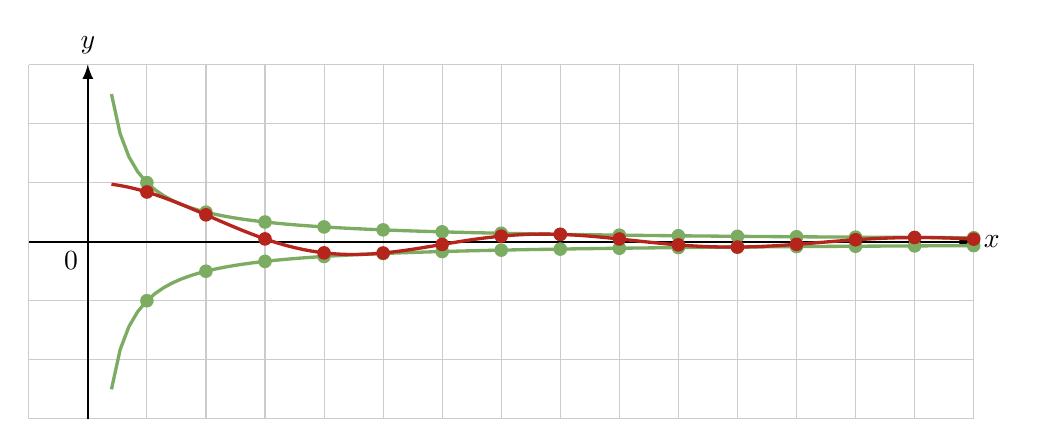
\begin{tikzpicture}[scale=0.75]
            \draw[thin,gray!40] (-1,-3) grid (15, 3);
            \draw[thick, ->, >=latex] (-1,0)--(15,0) node[right]{\(x\)};
            \draw[thick, ->, >=latex] (0,-3)--(0,3) node[above]{\(y\)};
            \draw (0, 0) node[below left] {0};

            \draw [OliveGreen!60, very thick, domain=0.4:15, samples=100] plot (\x, {1/\x});
    
            \foreach \x in {1,...,15} {
                \filldraw[OliveGreen!60] (\x, {1/\x}) circle [radius=3pt];
            }

            \draw [OliveGreen!60, very thick, domain=0.4:15, samples=100] plot (\x, {-1/\x});
    
            \foreach \x in {1,...,15} {
                \filldraw[OliveGreen!60] (\x, {-1/\x}) circle [radius=3pt];
            }
    
            \draw [BrickRed, very thick, domain=0.4:15, samples=100] plot (\x, {sin(\x r)/\x});
    
            \foreach \x in {1,...,15} {
                \filldraw[BrickRed] (\x, {sin(\x r)/\x}) circle [radius=3pt];
            }
        \end{tikzpicture}
        
        \caption{A demonstration of the squeeze theorem. The red curve represents the sequence \(v_n = (\sin{x})/x\). The green curves represent the sequences \(u_n = -1/n\) and \(w_n = 1/n\).}
        \label{fig:Ch05-squeeze-thm}
    \end{figure}
\end{itemize}





\subsection{What is a series?}

Consider the following sequence.
%
\[1, 2, 3, 4, 5, 6, \cdots\]
%
What happens when we add up the first \(k\) terms of this sequence?
%
\begin{align*}
    k = 1 \hspace{1cm} &{\color{BrickRed} \underbracket{1}_{1}} + 2 + 3 + 4 + 5 + 6 + \cdots\\
    k = 2 \hspace{1cm} &{\color{BrickRed} \underbrace{1 + 2}_{3}} + 3 + 4 + 5 + 6 + \cdots\\
    k = 3 \hspace{1cm} &{\color{BrickRed} \underbrace{1 + 2 + 3}_{6}} + 4 + 5 + 6 + \cdots\\
    k = 4 \hspace{1cm} &{\color{BrickRed} \underbrace{1 + 2 + 3 + 4}_{10}} + 5 + 6 + \cdots\\
    k = 5 \hspace{1cm} &{\color{BrickRed} \underbrace{1 + 2 + 3 + 4 + 5}_{15}} + 6 + \cdots
\end{align*}
%
Each of these sums is called a \textit{partial sum}, and together they form a new sequence, which in this case is the triangular numbers.
%
\[1, 3, 6, 10, 15, 21, \cdots\]

Whenever we take an existing sequence \((u_n)\) and compute its partial sums \(\left(\sum^{k=n}_{n=0} u_k \right)\) to form a new sequence, this new sequence is called a \textit{series}, denoted as \(\sum u_n\). The series of triangular numbers in particular can be described by the general term \(S_n = n(n+1)/2\). (This is a special case where we opt for one-based indexing!)\footnote{The formula can be proved as follows. Suppose we want to find \(S_n = 1 + 2 + 3 + \cdots + (n-2) + (n-1) + n\). This can be rewritten as \(S_n = n + (n-1) + (n-2) + \cdots + 3 + 2 + 1\). We can add these two equations together to get \(2S_n = (n + 1) + (n + 1) + \cdots + (n + 1) = n(n + 1)\). Dividing both sides by \(2\) yields \(S_n = n(n + 1)/2\).}

Now consider an arithmetic sequence
%
\[u_n = a + nd\]
%
where \(a = u_0\) is the first term. The series of this sequence is given by
%
\begin{align*}
    u_0 + u_1 + u_2 + \cdots + u_n &= a + (a + d) + (a + 2d) + \cdots + (a + nd)\\
    &= (n+1)a + (1 + 2 + \cdots + n)d\\
    &= (n+1)a + \frac{n(n+1)}{2}d \tag{using the formula for triangular numbers}
\end{align*}


What about the partial sums of a geometric sequence instead? Consider the sequence
%
\[u_n = ar^n\]
%
where again \(a = u_0\) is the first term. Denote the sum \(u_0 + u_1 + u_2 + \cdots + u_n\) as \(S_n\). We can write
%
\begin{align*}
    S_n &= a + ar + ar^2 + \cdots + ar^n\\
    rS_n &= ar + ar^2 + ar^3 + \cdots + ar^{n+1}
\end{align*}
%
Subtracting the bottom equation from the top one gives
%
\[(1-r)S_n = a - ar^{n+1}\]
%
which gives us the following formula for the series of a geometric sequence.
%
\[S_n = a + ar + ar^2 + \cdots + ar^n = \frac{a}{1 - r} (1 - r^{n+1})\]





\subsection{Convergence of a series}

Some series do not converge.
%
\[1 + 2 + 3 + 4 + \cdots \rightarrow \infty\]


However, some series do converge --- for instance, consider the following series. As the number of terms approach infinity, the sum approaches \(2\).
%
\[1 + \frac{1}{2} + \frac{1}{4} + \frac{1}{8} + \cdots = 2\]
%
To see why, we first note that this is a geometric series with partial sums
%
\begin{align*}
    S_n &= \frac{1}{1-\frac{1}{2}} \left(1 - \left(\frac{1}{2}\right)^{n+1}\right)\\
    &= 2 \left(1 - {\color{BrickRed} \left(\frac{1}{2}\right)^{n+1}}\right)
\end{align*}
%
As \(n\) approaches infinity, the term in red approaches zero, so the sum converges to \(2\). We can generalise this result as follows.
%
\begin{quote}
    \textbf{Convergence of a geometric series.}

    A geometric series \(\sum ar^n\) converges to \(a/(1-r)\) if \(-1 < r < 1\).

    In other words, we have
    %
    \[\sum_{n=0}^{\infty} ar^n = \frac{a}{1-r}\]
    %
    when \(-1 < r < 1\).
\end{quote}

This can be further generalised into what is called the \textit{ratio test} (also known as d'Alembert's criterion). But first, let us define the term \textit{absolute convergence}. A series \(\sum u_n\) is said to be \textit{absolutely convergent} if the series \(\sum \abs{u_n}\) converges.

And now, the ratio test.
%
\begin{quote}
    \textbf{Ratio test for convergence of a series.}

    To determine whether a series \(\sum a_n\) converges (assuming \(a_n \neq 0\) for all \(n\)), we consider the sequence of ratios \(\dfrac{\abs{a_{n+1}}}{\abs{a_n}}\).
    %
    \begin{align*}
        \lim_{n \to\infty} \frac{\abs{a_{n+1}}}{\abs{a_n}} > 1 &\implies \text{the series diverges}\\
        \lim_{n \to\infty} \frac{\abs{a_{n+1}}}{\abs{a_n}} < 1 &\implies \text{the series converges absolutely}\\
        \lim_{n \to\infty} \frac{\abs{a_{n+1}}}{\abs{a_n}} = 1 &\implies \text{no conclusion reached}
    \end{align*}
\end{quote}

For example, consider the series \(\sum (n+1)/2^n\). Applying the ratio test, we consider the limit
%
\begin{align*}
    \lim_{n \to \infty} \frac{(n+2)/2^{n+1}}{(n+1)/2^n} &= \lim_{n \to \infty} \frac{n+2}{2(n+1)}\\
    &= \lim_{n \to \infty} \frac{(n+1) + 1}{2(n+1)}\\
    &= \lim_{n \to \infty} \frac{(n+1) + 1}{2(n+1)}\\
    &= \lim_{n \to \infty} \left(\frac{1}{2} + \frac{1}{2(n+1)}\right)\\
    &= \frac{1}{2}\\
    &< 1
\end{align*}
%
which means the series is absolutely convergent. Since all terms are positive, the series is also convergent.

We also have a comparison test for series convergence. Consider two series \(\sum a_n\) and \(\sum b_n\), where \(a_n, b_n \geq 0\). Then,
%
\begin{itemize}
    \item If we have \(a_n \leq b_n\) and \(\sum b_n\) is convergent, then \(\sum a_n\) is also convergent (smaller than a convergent series).
    \item If we have \(a_n \geq b_n\) and \(\sum b_n\) is divergent, then \(\sum a_n\) is also divergent (larger than a divergent series).
\end{itemize}

As an example, consider the series \(\sum 1/(2^n + 1)\). We can easily show that \(1/(2^n + 1) \leq \frac{1}{2^n}\). Since the series \(\sum 1/2^n\) is convergent, the series \(\sum 1/(2^n + 1)\) is also convergent.

Similarly, consider the series \(\sum_{n \geq 3} (\ln{n})/n\). When \(n \geq 3\), we have \(\ln{n} \geq 1\), so \((\ln{n})/n \geq 1/n\). Since the series \(\sum 1/n\) is divergent, the series \(\sum (\ln{n})/n\) is also divergent.